%section: Ransomwares and ransomware attacks
%last subsection: how to get infected
    \subsection{Encryption mechanism: how do ransomware work}
        Once the malware starts running on target computer, it generates a random symmetric key\footnote{used both to encrypt and decrypt information}, usually one per file, and it encrypts each file with it.\\
        The symmetric key itself it's encrypted with a public key, of an asymmetric key pair generated on the server of the group that runs the malware. The private key is stored on the server, and it will released only when the ransom is payed.\\
        Most of this process is automated: when cryptocurrencies are transferred to the criminals' address, the server releases the key associated to it.
        Different keys to allow the attackers to decrypt only a part of the samples to demonstrate that they can do it.
\section{Indirect monetization: Botnets}
    The word botnet comes from the words \textit{robot} and \textit{network}. A botnet is composed by few hundreds to millions of infected devices which run some sort of malware they got by opening an infected email attachment, by plugging an infected USB drive, visiting an infected website \textit{(these are examples of ways to get infected)}\\
    Each botnet has a \textbf{botmaster} who controls and rents it out to perform tasks \textit{(denial of service, spamming, phishing campaigns, crypto mining \dots)}, and his only objective is to earn money by renting them.\\
    The significant challenge with this type of crime is that each bot per-se is not dangerous for the machine itself, but for other machines, and since the cost of cleaning up a machine falls on its owner, some can decide to not do anything about. This cost can be seen as a small fee to be payed by \textit{the community} to get everybody safe. Like a vaccination, some cases of infected machines are not a big trouble for the community, while a lot of them can be really dangerous for everybody.
    \subsection{Rise of the bots}
        Back in the days botnets were used to control IRC chats \textit{(see IRC wars)}. Then instead of using the compromised machines to control the chat, botmasters started to use the chat to control the bots.\\
        In 1999, there was one of the first DDoS attacks, which was against University of Minnesota and used at least 227 bots.\\
        In the 2000s DDoS attacks against high profile websites \textit{(Amazon, CNN, eBay \dots)} got huge media coverage.
\newpage
    \subsection{Geolocalization of botnets command and control}
        \begin{figure}[ht!]
            \centering
            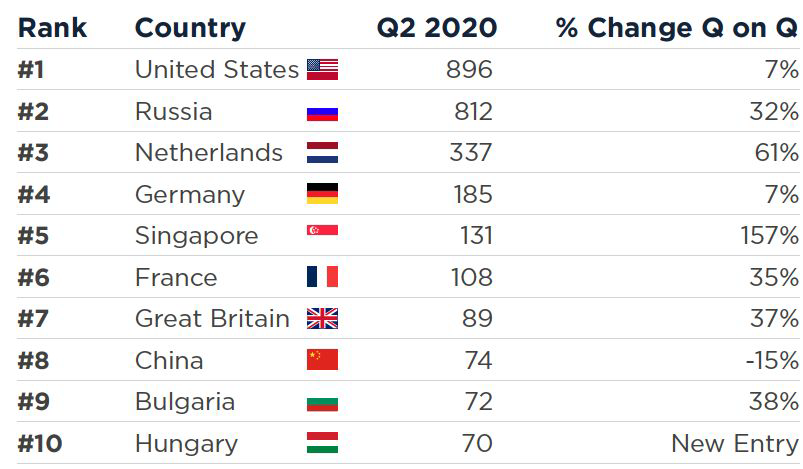
\includegraphics[width=0.6\linewidth]{chart.png}
        \end{figure}
        This chart shows the number of new botnet C\&Cs detected by \textit{Spamhaus} in the second quarter of 2020, and the increase wrt the first one.\\
        By keeping in mind the \textit{observation bias}, we can also introduce another kind of bias which is called \textbf{heatmap effect}: we're biased on the density of the population and on how much data we collect from a certain country.\\
        In this kind of charts we'll always have U.S.A. on top, because there's more penetration in the internet, and also this kind of things is tracked. While we'll have less data from less technological advanced states or \textit{perfectly democratic countries} like Russia or the P.R.C. which can result in lower positions while in reality being the first ones.\\
        Here we see an important increase of C\&C from The Netherlands:
        \begin{itemize}
            \item it is possible that \textbf{something is on}
            \item or simply that some Netherlands organization decided to participate in this data collection feeding a lot of \textit{new} data
        \end{itemize}
        Funny thing about Russia and P.R.C: Russian people hack russian computers too, while P.R.C citizens don't hack into their fellows machines.
\newpage
    \subsection{Type of (botnet) malware families}
        \begin{figure}[ht!]
            \centering
            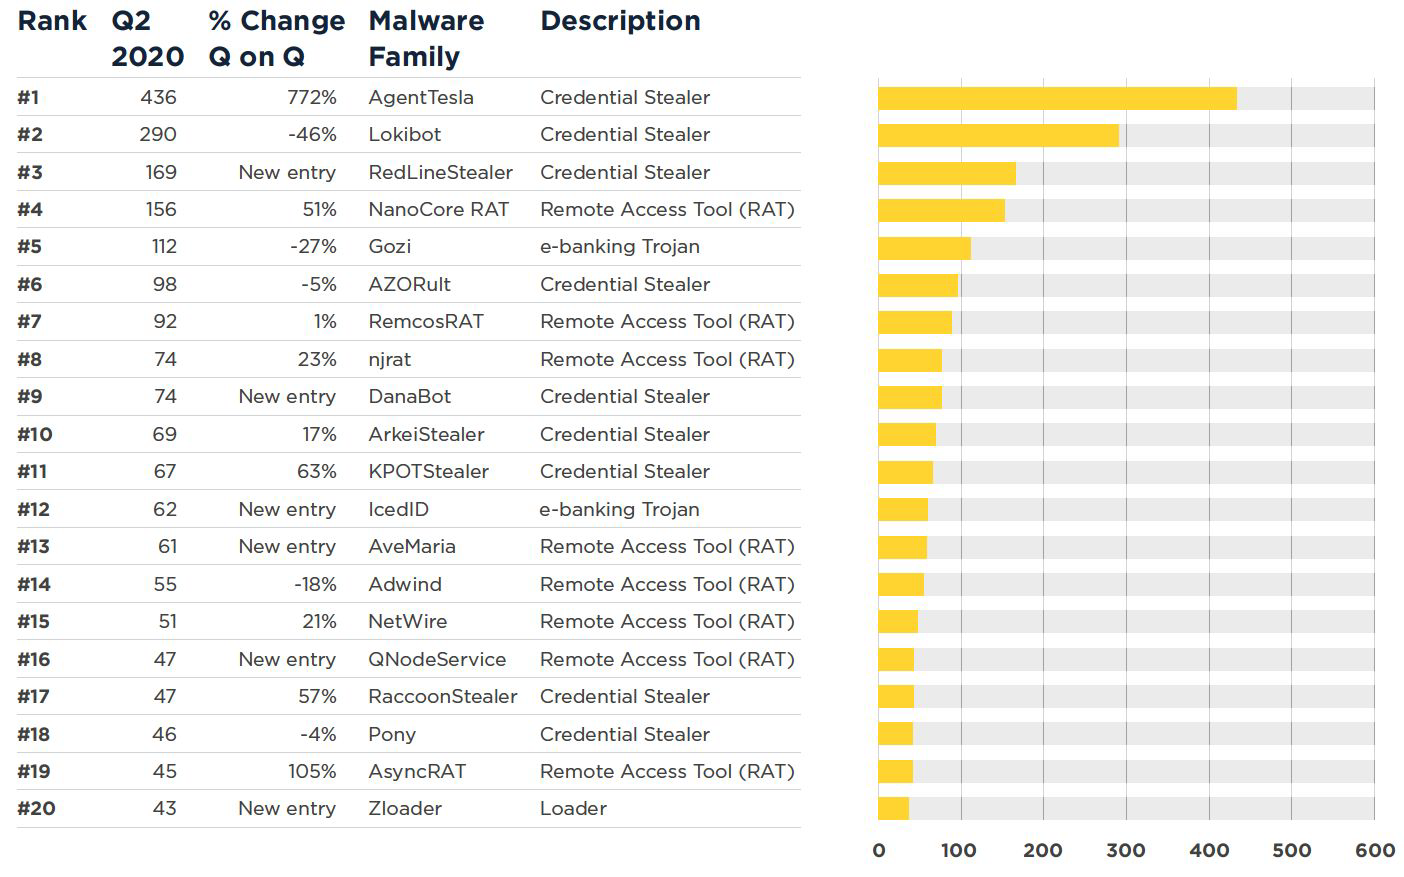
\includegraphics[width=0.6\linewidth]{families.png}
        \end{figure}
        Every botnet in general can be used to do any sort of things, but they're used to do only one of them:
        \begin{itemize}
            \item \textbf{Credential Stealers:} used to steal sensitive credentials.
            \item \textbf{Banking Trojans:} credential stealers specifically designed to perform stealing of bank accounts information. \textit{(Gozi is the most common one, Zeus the most important one)}
            \item \textbf{Remote Access Tools:} basic botnet oriented malware, which allows to control a computer in order to perform whatever.
            \item \textbf{Loaders:} specifically designed to allow a botmaster to load a program of whatever sort on a computer. Maybe a client ask you to install a certain malware on a lot of computers, and you can do it with a loader.
        \end{itemize}
        We talk about families because there are criminal groups that only develop their source code, and who performs the attacks buys the code and personalizes it for the specific purpose they need.\\
        So we can consider three businesses: how to develop them, how to configure them, how to use them.\\
        There is a market for services related to malwares and cyber attacks \textit{(cybercrime as a service, underground market...)} structured around the needs of cyber criminals. This market is fueled by the money that these schemes make. Some of these money pays for the tools used to make that money.
\iffalse
SLIDE 
    someone stole money from 104000 taxpayers.
    What is the value of someone personal datas that you exchange with agenzia delle entrate?
    You can sell identities on the black market. Worth because them can be used for fraud, open bank accounts used for money laudery.
    The more they're useful, the more they are worth.
    Worth 50 dollars for you that sell it, who pays is going to use them for fraud which is worth more.
    Market fueled from an enormous amount of money that people stole.
SLIDE 23

    another way in which malwares are installed
    drive by download, exploit breaks your browser and executes code on your machine. This requires your browser to be vulnerable and for you to visit the website which uses it.
    people compromises or run websites like porn, streaming, cracks of programs.
    you're not scared of the strange url if you are in need to see streaming, download crack, in contrast with amazon if you buy shoes.
    you can also place the "trap" in a legitimate website.

    In reality you'll endup in a series of redirect chain 
    In that redirection chain you endup in the exploitation pack for your browser:
        there is people selling this service kit to try 10-12 exploits tipo abbonamento 10.000€ mese 

SLIDE 24
    Advertisement of someone selling, 

SLIDE 25(?)
    Dashboard of black hole: exploitation as a service
    black hole ended in 2013 because the guy was arrested.

    These people just buy exploits, because they just can earn 10s millions per month and pay exploit hackers to develop them.

SLIDE 25:
    these ecosystems can exists because some of the activites done are not illegal. Developing exploits per se is not illegal, selling one is not illegal, the usage of them may be or may be not illegal.
    Even the services related to the configuration of malware are not, execution and operation may be.
    If you're sufficiently shielded and you run in countries that cannot persecute you, we can know even name and surname but people cannot be arrested.

    packers develop things used in malwares, 
    lot of other affiliates: quality assurants change them to not be detected from antiviruses
    bulletproof hosting: hosts that kind of close an eye, for instance russian business network hosted whatever.
    borderline organization with lot of regular customers, and some bad ones
    
    botnets are both enabler or attacks
    + the part of money laundering
SLIDE 26
    someone looking to buy vulnerabilites.
SLIDE 29
    monetization takes a lot of forms:
        people buying and selling cc numbers for 30\$ of sure and safe money instead of laundering.
        an example is buying apple computers or expensive things.
        They sell a volume of these for little sure and easy money.
        
        To make the card i bought for 30 in something more valuable
            travel industry: ethnic travel agencies are those that work with immigrants
            lot of planes to fill-up 
            partially tourists and business people
            part of them sold in blocks to people who travel back to their home countries for a low price.
            legal business.

            This creates possibility for a fraud:
                these people are used to buy in cash the tickets for a much lower price than you can find online.
                if you buy tickets with a stolen credit card from a regular travel agent and resell them for cash in a poor neighbor as a ethnical travel agent
                you make less money, if person find out 
                you have sold the ticket for a lower secure money.
                if buyer is very unlucky gets to the airport and gets arrested.

    If you detach others from the picture (online), it's easier to commit crimes: example steal a car vs steal a movie.
    lot of cyber criminal would not do the same thing in the real world
    different PERCEPTION.
    This makes crime happen more often online,
    lot of crime enablers
    ethical people understand consequences of your actions.

Telephone of Khashoggi was infected with spywares.
Who sold the eploits for this phone to let the spyware installed would never had killed Jamal
The exploit maybe or not may not be used in that way.
this permits more people in participate

SLIDE 31 MONEY MULES AND MONEY LAUNDERY
    most cybercrime end up with a digital form of money.
    Your problem is to bring this in a form which is not linked to the crime.
    On a certain level this may sound easy, in general it is not because most of the transfers leave a trace.
    The real moment in which a criminal brakses the chain of traceability is the moment when cash turn physical cash or goods and go back digital again.

    Some of the schemes are traditional:
        pay invoice to a company somewhere in the world, runs some processes, pays other companies... 

    Particular cyber crime one:
        use of money mules: they're traditionally accomplished, they know what they're doing, they have not so much to luse
        they open bank accounts, receive the money and hand cash to somebody
        
        some of them open account with different identity, and to catch them you need to do while they whitdraw. More difficult.

        Nigerian prince:
            ask you money in order to get more money, cost 500 dollars to get 1 billion
            until you realize that you have been scammed they keep asking you money.

            A variant is connected to the money mule.
                you actually get the promised money, i give you money, withdraw them and send them phisically with money transfer to someone
                keep 30\%
                Or send the money in an envelope to a postal box in kazakhstan

                Money arrive in your bank account from bank accounts of compromised people.
                At a certain point they arrest you.
                Good lawyer: you've been cheated. Ridai il 30 che ti sei tenuto e ripaga il 70
                Bad lawyer: you get persecuted.

        Considera RICETTAZIONE: apple computer sold at 40\% in meno....

        points, virtual currency of games has been used for this...  

        If you are a cyber criminal with crypto you need an exchange which is not any exchange but a stronzo one.


\chapter{Cryptocurrencies: abuses and forensics}
    we talk about them in the way they are used in cybercrime.

    Bitcoin is the attempt to create electronic cash.
    cash has a lot of properties that you would replicate, in the digital world usually you don't have these properties.

    electronic distributed ledger (node of where all the transaction happened)
        no central authority
        need to solve a problem which is very hard
        problem of byzanine consensus
        blockchain enables the creation of distributed ledger.
        used to run bitcoin, but you can use any other ledger to run blockchain

SLIDE 4
    in the bitcoin world every user uses a wallet (the way they were designed originally)
    in btc the concept of cryptographic pair of keys can hold a certain amount of btc
    by using the keys you can use/send those money
    what uses them is called wallet.

SLIDE 5
    bitcoin address is alphanumeric string which identifies a point where you can send bitcoin
    and where them can start from.
    In order to know how much btc are in that key you need to go to the origin of all the transactions and track the flow of them to understand how much of them are there now.

    Not really efficient but can run without central authority 
    The only reason for using a blockchain is if it is really so important to get a way out of a central authority
    it is the less efficient thing ever but it has a way out of central authority.
    for any other reason it doesnt' make sense.

    WE WANT TO DO TRANSACTION ON A LEDGER WITH NO AUTHORITY, WHE USE THIS SHITTY TECHNOLOGY
SLIDE 6
    as soon the transaction is on the immutable ledger the money are on the other address.
    How do we ensure that this is the only transaction done with that bitcoin 
    we need to have a consolidated immutable ledger
    with a central authority this would be easy.
    how do we agree on a ledger which cannot be back modified?

    slide 7
        certain btc associated with your public key
        joe signs a transaction which moves them to alices' wallet.

        I need to have an history that cannot be modified
            Joe could unsign the key. How do we do?

        Transactions are put in a block, block linked in a so-called block chain (linked list)
        we want this list to be immutable

        Mining:
            Solves 2 problems:
                ensuring that the list cannot change 
                generate bitcoin

                we seal the block and get a little btc in reward, and when we seal the block we tell everyone were we want to send the reward

                mining is a very computational demanding activity
                    hash function 
                    collect transaction, put them in the block, put there a destination for a reward
                    bruteforce the block in a way that the hash of the block has a certain number of zeros to start with.
                    This is difficult, the more zeros at the beginning, the more difficult for a miner to find the right combination.
                    Miners are using computational power to trying to find the right solution, once they find it they publish the solution.
                    At this point the other miners, look at the transaction that are not in a block yet, try to put them in the next block and try again.
                    The more computational power you put, the faster you will get to the solution.

                    The difficulty increases more and more, the reward got smaller and smaller but btc value gets larger and larger.

                    block = set of transactions + reward location which a sha256 with a certain number of zeros.

                    After I found a solution, the new block must be linked to this one ... mancaun pezzo 13.56 sul next hash 


                    Sooner or later two entities get a solution at the same time or more or less. What happens?
                    For some people chain ends with block a and some with block b, do i append to a or to b?
                        what happens is a fork
                        slide 13,14 ...  
                            alternative ending of the chain
                            some nodes see the 1st, some the 2nd.
                            you start from there and search the next one.
                            you can see now two different blockchains.
                            sooner or later someone finds a solution
                                who mines on the green blockchain fount the purple solution
                                    the rule now is that the true blockchain is the longest one.
                                        purple block is one ahead, i'm no more in the true one. 
                                        it doesn't make more sense to try again the red one.
                                        give up and go to the shortest.
                                    
                            This is done because in order to revert a payment you'd need to go back on your block, go ahead mining until your blockchain is now the longest one
                            means that you compete with all the others.

                            Blockchain solves the problem of central authority by making people to do useless thing 





\fi